\documentclass[11pt,letterpaper,boxed]{pset}

\usepackage[margin=0.75in]{geometry}
\usepackage{ulem}

\name{Name: \rule{2.5cm}{0.15mm}}
\assignment{Box \# \rule{1.5cm}{0.15mm}}
\class{MATH065 HW10}
\duedate{05 June 2019}


\begin{document}

    \problemlist{MATH065 HW10}

    \begin{problem} [Exercise 1. ]
        Consider the nonlinear  system
        
        \begin{eqnarray*}
            \dot{x} & =& y-x \\
            \dot{y} &=& 2xy-2y 
        \end{eqnarray*}
        
        \begin{itemize}
            \item[(a)] Plot the nullclines for this system. Draw arrows on your nullclines indicating the direction of motion for states on the nullcline. 
            \item[(b)] Determine all equilibrium points. 
            \item[(c)] Compute the Jacobian matrix $D\mathbf{f}$ at each equilibrium point, and find the associated eigenvalues and eigenvectors for the linearization at each equilibrium point. 
            \item[(d)]  Assuming the linearization is accurate use your information from part (b) to sketch the phase portrait near each equilibrium point. You don't need to draw the entire phase portrait, just what your linear models predict the system looks like near the equilibrium points.   Classify each equilibrium point by type (e.g., nodal sink, nodal source, spiral sink, etc.) and stability (stable, asymptotically stable, or unstable).
        \end{itemize}
    \end{problem}
    \newpage
    
    
    \begin{problem} [Exercise 2. ]
        (Competing Species) 
        Consider a model for interactions between rabbits, $x(t) \geq 0$, and  hares, $y(t) \geq 0$ (measured in arbitrary units):  
        
        \begin{eqnarray*}
            \dot{x} & =& x (4 - x - 3y) \cr
            \dot{y} &=& y (4- 3x -y) 
        \end{eqnarray*}
        
        \noindent
        \parbox{0.5\textwidth}
        {
            \[ 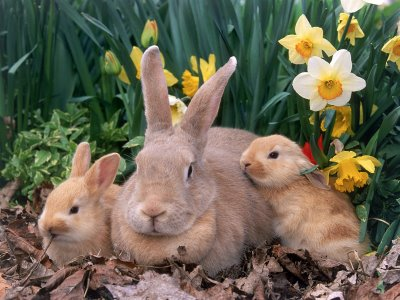
\includegraphics[width=0.33\textwidth]{rabbits}  \]
            \[  x(t) \]
        }
        \parbox{0.5\textwidth}
        {
            \[ 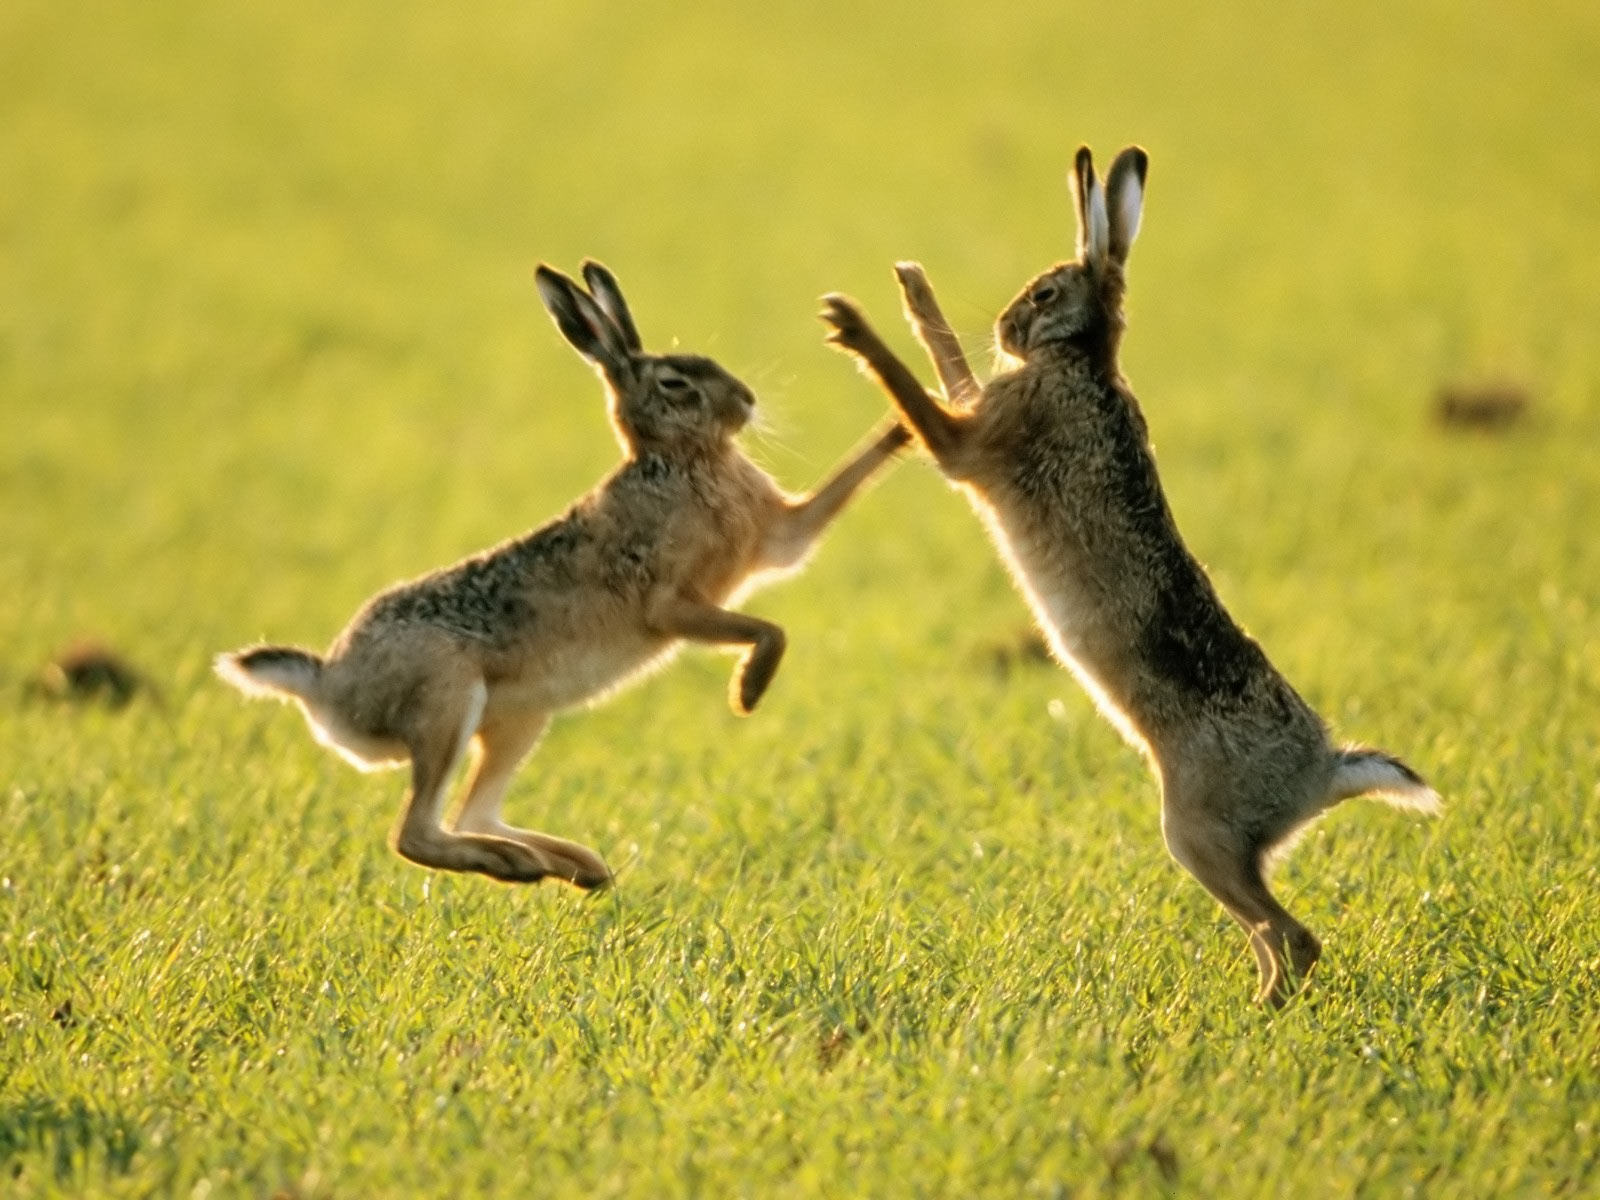
\includegraphics[width=0.33\textwidth]{hares}  \]
            \[  y(t) \]
        }
        
        \begin{enumerate}
            \item[(a)] Plot the nullclines and determine all equilibrium points. Hint: There are four equilibrium points. 
            \item[(b)] Linearize the system at each equilibrium point, and find the eigenvalues and eigenvectors of the resulting linear system. Classify each equilibrium point by type  and stability.
            \item[(c)] Assuming the linearization is accurate, use your results from (b) to sketch the phase portrait (you can check with pplane or other software to help connect your local linear information more globally). Recall $x,y \geq 0$, so you only need to plot the orbits in the first quadrant. Note: be sure to draw a healthy size first quadrant so you can clearly indicate the various details.
             \item[(d)] (principle of competitive exclusion) Assuming that we start with a nonzero population of rabbits and hares, what does the model predict for the populations over large time (i.e., where do the orbits end up)?    
        \end{enumerate}
    \end{problem}
    \newpage
    
    
    \begin{problem} [Exercise 3.]
        (SIR model) The state variables  $S$ and $I$  in the SIR model form a closed subsystem, so to analyze the SIR model it is sufficient to study the two-dimensional system
        
        \begin{eqnarray}
            \label{s}
            \dot{S} & = & -\alpha S I \\
            \label{i}
            \dot{I} & = & \alpha S I - \beta I 
        \end{eqnarray}
        
        We are only concerned with the dynamics  in the first quadrant ($S \geq 0, I \geq 0$) with $S \leq 1$ and $I \leq 1$ (in general $I << 1$). 
        
        \begin{enumerate}
            \item[(a)] In the previous assignment we found any point of the form $(S_0,0)$ is an equilibrium point. Show that the linearization at any such point has $0$ as an eigenvalue.  Show that the other eigenvalue is positive when $S_0 > \frac{\beta}{\alpha}$ and negative when $S_0 < \frac{\beta}{\alpha}$.  
            \item[(b)] Let $\beta =1$ and $\alpha = 2$. Use pplane (or some other software) to plot some sample  phase portraits  assuming $0 \leq S \leq 1$. Choose your axes to ensure all the key behavior of the model is demonstrated in your figure. 
            \item[(c)] Suppose the system is perturbed from the disease free equilibrium state $(1,0)$ (e.g., if the initial state is $(0.999,0.001)$, modeling the introduction of the disease into a population that is all susceptible), what does the model predict for the values of $S(t)$ and $I(t)$ as $t \to \infty$? 
        \end{enumerate}
    \end{problem}
    \newpage
    
    
    \begin{problem} [Exercise 4. ]
        (\textbf{Chemical Oscillator}) The Brusselator Model is a model for chemical oscillations (including biological oscillations):
        
        \begin{eqnarray}
            \label{al2}
            x' & = & a - b x + x^2 y - x \\
            \label{be2}
            y' & = & b x - x^2 y
        \end{eqnarray}
        
        where $a > 0$ and $b > 0$. We assume $x \geq0$ and $y \geq 0$ (since they represent chemical concentrations). 
        
        \begin{enumerate}
            \item[(a)] Use a calculator or graphing program to plot the nullclines in the first quadrant (you can assume $a=b=1$). Draw arrows on your nullclines indicating the direction of motion for states on the nullcline. 
            \item[(b)] Show the system has a unique equilibrium point and this equilibrium point is unstable when $b > 1 + a^2$. Hint: By the $2 \times 2$ zoology of phase portraits we know an equilibrium point is unstable when the trace is positive. 
        \end{enumerate}
    \end{problem}
    \newpage

\end{document}
